\chapter{Cloud-Edge Continuum}
Cloud computing, even if it provides potentially unlimited storage and processing capabilities, has three key issues which may be critical in some situations:
\begin{enumerate}
   \item Latency
   \item Internet connection Required
   \item Lots of Data over the network
\end{enumerate}
Conversely, relying on an infrastucture on the "\textit{Edge}", i.e. close to the IoT device, offers low latency but limited storage and processing capabilities.


So the key idea of the \textbf{Cloud-Edge Continuum} is to extend the cloud towards the IoT world into a\ul{\textit{distributed} and \textit{heterogenous}
infrastructure} to get the best of both Cloud and Edge approaches.\\
Hence, applications should be \textbf{microservice}-based and \textbf{containerised}, allowing them to be deployed on a \textit{continuous Cloud-Edge infrastructure}.


\section{Placing applications}
There are many issues the infrastructure has to manage;
\begin{enumerate}
   \item \textbf{Hardware} and \textbf{Software} requirements
   \item \textbf{Data Gravity}
   \item \textbf{Security}\\
   Need to match application’s security requirements
   with infrastructure’s security capabilities
   Need to model (non-monotonic, conditionally transitive)
   trust relations among different stakeholders
   \item \textbf{Sustainability}
   \item \textbf{Infrastructure}
\end{enumerate}

Placing applications in the Cloud-Edge Continuum is challenging and \textit{\textbf{NP}-Hard};
approaches to solve the problem include \texttt{ML}, \texttt{MILP}\footnote{Mixed-Integer Linear Programming}, \textit{Declarative Reasoning} supported by an \textit{Inference Engine}.

\section{Managing applications}
Infrastructure and applications will most-likely mutate throughout time,
so the eventual changes must be managed, and in order to do so,
they must \textit{both} be \underline{monitored}.

There must a be a process of \textit{continuous reasoning}, to exploit compositionality to differentially analyse a large-scale system:
\begin{itemize}
   \item mainly focusing on the latest changes introduced in the system,
   and
   \item re-using previously computed results as much as possible
\end{itemize}

\begin{figure}[htbp]
   \centering
   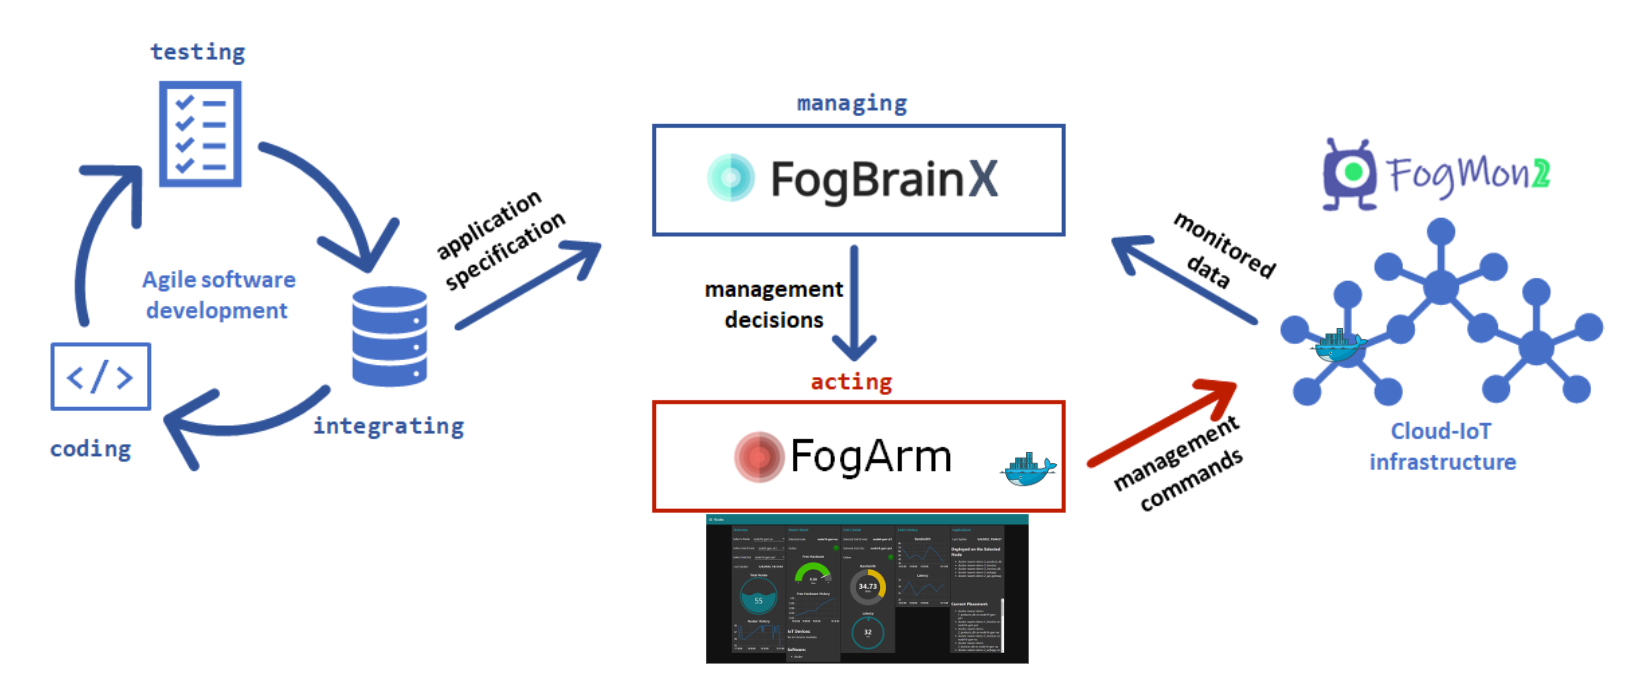
\includegraphics{images/edge_reasoning.png}
   \caption{Monitoring $\longrightarrow$ reasoning $\longrightarrow$ enacting}
   \label{fig:edge_reasoning}
\end{figure}

\begin{itemize}
   \item Osmotic Management
   \item Decentralized management (bacteria-inspired)
   \item 
\end{itemize}